\documentclass[./einleitung.tex]{subfiles}
\usepackage{float}
\usepackage{float}
\usepackage{float}
\usepackage{float}
\begin{document}
    \section{Die Nutzung des \acrshort{lsp}}
    \subsection{Installationsmöglichkeiten}
    Der \acrshort{lsp}-Server benötigt keine zusätzlichen Strukturen und kann direkt als Datei ausgeführt werden.
    Deshalb ist die normale Vorgehensweise das Ablegen des \acrshort{lsp}-Servers in einem Zentralen Server und das Hinzufügen des Pfades zu dem Umgebungsvariablen.
    Im Beispiel wurde die Datei zu `dmflsp' umbenannt, damit der Name genauer das Programm beschreibt und nicht mit anderen \acrshort{lsp}-Server kollidieren kann.\\
    \begin{figure}[h]
        \centering
        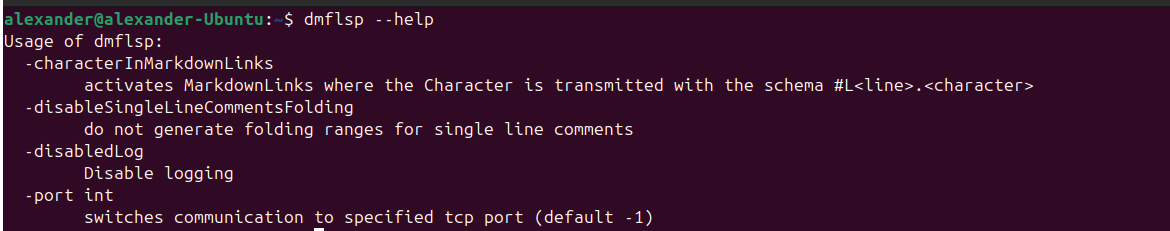
\includegraphics[width=\linewidth]{bilder/screenshot-lsp-help}
        \caption{Aufruf des \acrshort{cli} des \acrshort{lsp}-Servers}
        \label{fig:screenshot-lsp-help}
    \end{figure}\\
    Es gibt Editoren die eine native Anbindung eines \acrshort{lsp}-Servers ermöglichen.
        {\footnotesize TODO Zed Besspiel }
    \subsubsection{Intellij}
    Intellij unterstützt nur wenige \acrshort{lsp}-Funktionen ohne zusätzliche Plugins.
    Mit von `lsp4ij' können \acrshort{lsp}-Server direkt in der Oberfläche konfiguriert werden.\\
    \begin{figure}[h]
        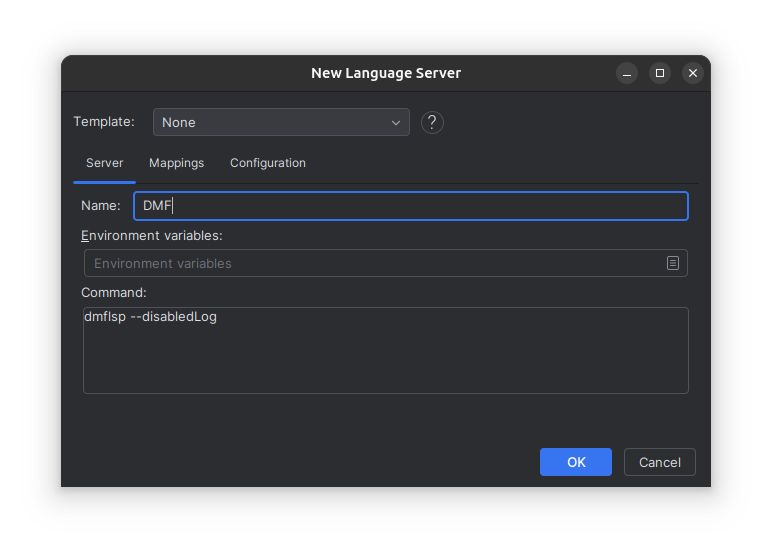
\includegraphics[width=\linewidth / 2]{bilder/screenshot-add-lsp-lsp4ij}
        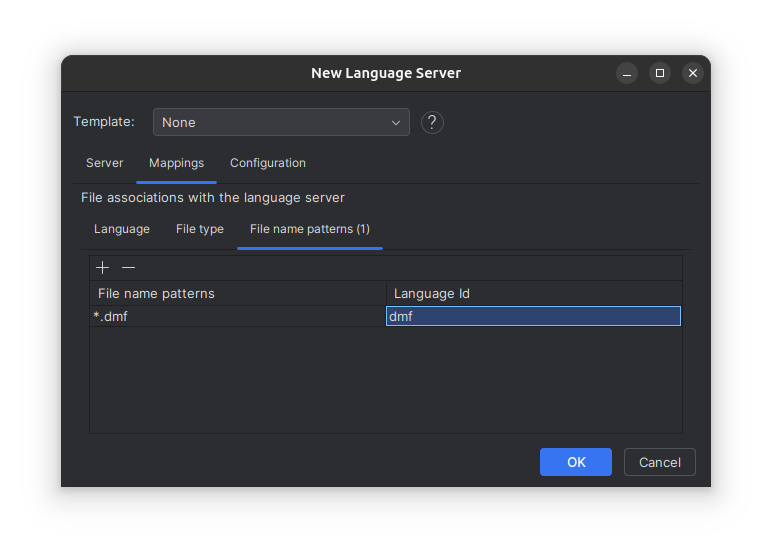
\includegraphics[width=\linewidth / 2]{bilder/screenshot-file-mapping}
        \caption{lsp4ij Konfiguration}
        \label{fig:screenshot-add-lsp-lsp4ij}
    \end{figure}\\
    Um diese Konfiguration automatisch anzulegen und den Dateien ein passendes Icon zu geben, kann das Intellij-Plugin für das \acrshort{dmf} verwendet werden.
    Es enthält die verschiedenen Versionen des Servers und kann sie automatisch an den konfigurierten Pfad ablegen.
    Der Pfad zum \acrshort{lsp}-Server kann entweder in den Einstellungen des Plugins oder über die Umgebungsvariable `DMF\_LSP' konfiguriert werden.

    \subsubsection{Visual Studio Code}
    Um den \acrshort{lsp}-Server in Visual Studio Code nutzen zu können, wird die Erweiterung für das \acrshort{dmf} benötigt.
    Dieses enthält die Logik zum Verbinden zum Server und die verschiedenen Versionen.
    Die benötigte Version kann direkt ausgeführt werden und benötigt keine zusätzliche Konfiguration.\\
    Im Gegensatz zu den bisherigen Konfigurationen nutzt die Visual Studio Code Erweiterung eine \acrshort{tcp}-Verbindung.


    \subsection{Funktionen im Editor}
    Während des Bearbeitens der Modelle können die Funktionen des \acrshort{lsp}-Servers genutzt werden.
    In diesem Abschnitt werden die Funktionen präsentiert.
    
    \subsubsection{Einfärbung des Textes}
    Mithilfe der semantischen Token kann der Editor den Text der Modelldatei einfärben.
    Da der Server nicht die Farbe, sondern nur die Funktion, vorgibt, wird der Text anhand der Einstellungen der Entwickler*innen eingefärbt.
    \begin{figure}[H]
        \centering
        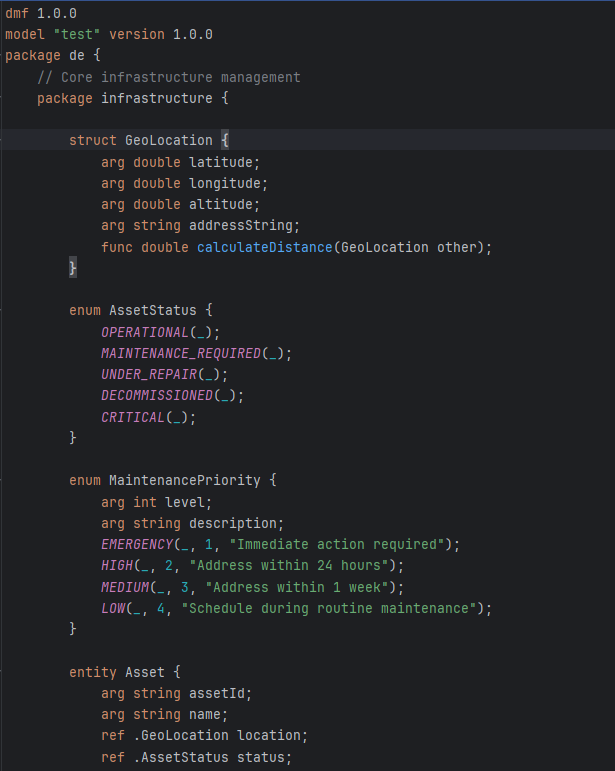
\includegraphics[width=\linewidth / 2 - 1em]{bilder/semanticIntellij}
        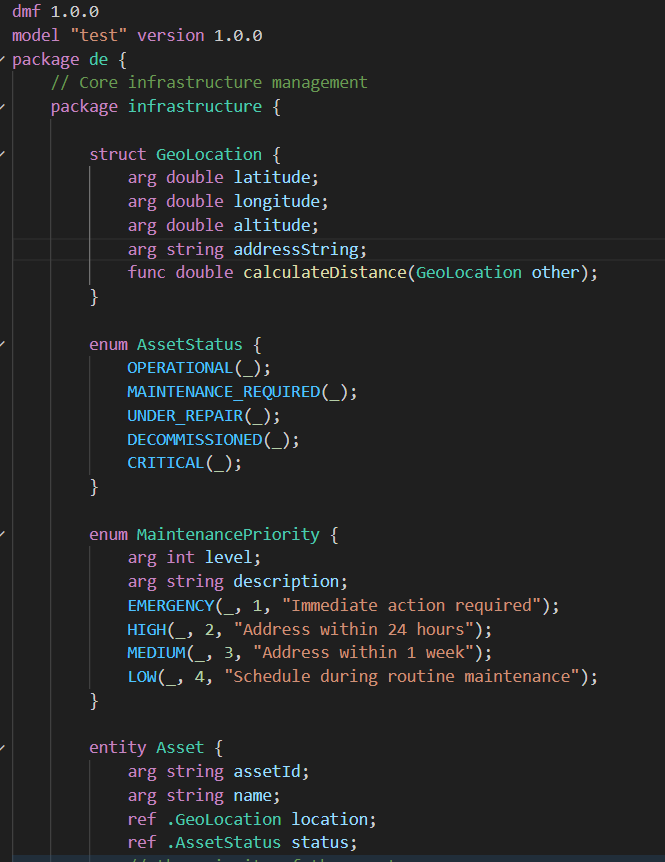
\includegraphics[width=\linewidth / 2 - 1em]{bilder/semanticVscode}
        \caption{Eingefärbte Modelldateien in Intellij und Visual Studio Code}
        \label{fig:semanticintellij}
    \end{figure}

    \subsubsection{Diagnosen}
    Wenn der Fehler in der Datei existieren werden diese automatisch im Editor markiert.
    Es wird auch eine Beschreibung und die detaillierte Beschreibung, welche auch im Generator ausgegeben wird, übertragen.\\
    Die Darstellung wird von der \acrshort{ide} übernommen.
    In Intellij und Visual Studio Code wird die Hover-Beschreibung zusätzlich angezeigt.\\
    \begin{figure}[hH]
        \centering
        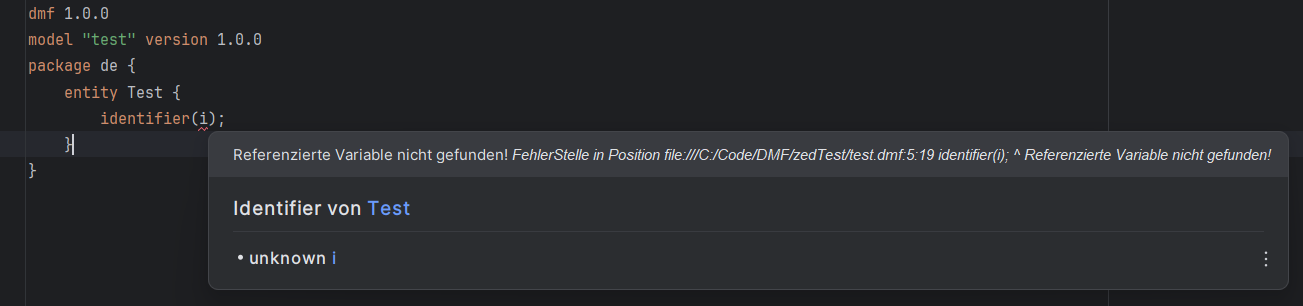
\includegraphics[keepaspectratio,height=8em]{bilder/markierung-fehler-intellij}
        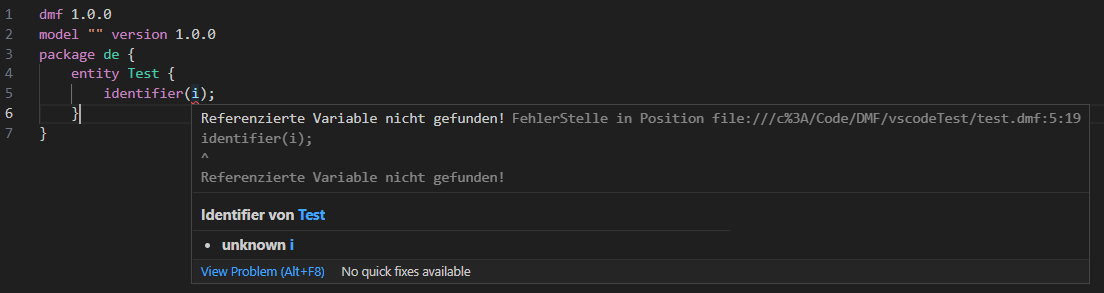
\includegraphics[keepaspectratio,height=8em]{bilder/markierung-fehler-vscode}
        \caption{Beispiele aus Intellij und Visual Studio Code}
        \label{fig:markierung-fehler-intellij}
    \end{figure}

    \subsubsection{Hover-Beschreibungen}
    Um Informationen über ein Element bereitzustellen, kann mit dem Mauszeiger über einem Element gehovered werden.
    Für alle PackageElemente, EntityIdentifier, Argumente, Referenzen, MultiReferenzen und Kommentare können Beschreibungen angezeigt werden.
    Mithilfe von Links in den Beschreibungen kann direkt zum erwähnten Element navigiert werden.
    \begin{figure}[H]
        \centering
        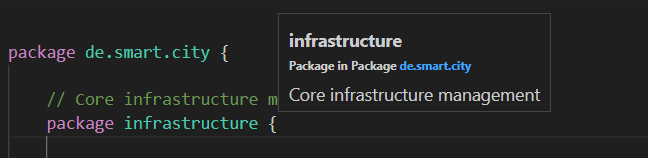
\includegraphics[height=5em]{bilder/hover-package}
        \caption{Beschreibung eines Package Elements}
        \label{fig:hover-package}
    \end{figure}
    Bei PackageElementen enthält die Beschreibung den Kommentar des Elements sowie das Package, in dem es liegt.
    \begin{figure}[H]
        \centering
        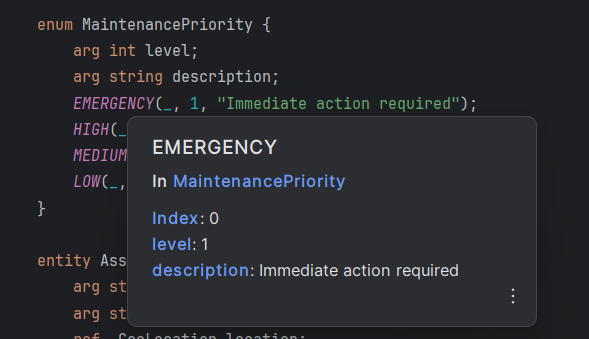
\includegraphics[height=7em]{bilder/hover-enum-entry}
        \caption{Beschreibung einer Enum Konstante ohne Kommentar}
        \label{fig:hover-enum-entry}
    \end{figure}
    Die Beschreibung von Enum Konstanten enthält das Enum, falls vorhanden den Kommentar und die Argumente des Enum mit den Werten der Konstante.
    Der erste Wert ist der Index, welcher in der Datenbank gespeichert wird.
    \begin{figure}[H]
        \centering
        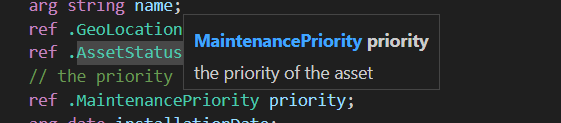
\includegraphics[height=5em]{bilder/hover-referenz}
        \caption{Beschreibung einer Referenz}
        \label{fig:hover-referenzen}
    \end{figure}
    Referenzen enthalten den Kommentar sowie den Typen und Namen der Variable.
    Argumente und MultiReferenzen verhalten sich gleich.
    \begin{figure}[H]
        \centering
        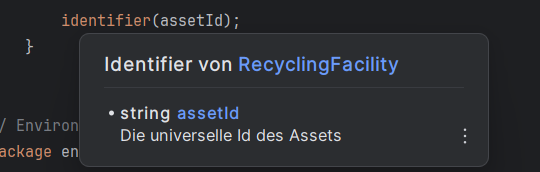
\includegraphics[height=7em]{bilder/hover-entity-identifier}
        \caption{Beschreibung eines Entity Identifiers}
        \label{fig:hover-entity-identifier}
    \end{figure}
    Bei einem Entity Identifier werden die referenzierten Variablen ihren Kommentaren angezeigt.

    \subsubsection{Referenzen}
    In den \acrshort{ide}s können die Referenzen aufgerufen werden.
    Der \acrshort{dmf}-\acrshort{lsp}-Server findet Referenzen, Deklarationen und Verwendungen in Parametern und EntityIdentifier.
    \begin{figure}[H]
        \centering
        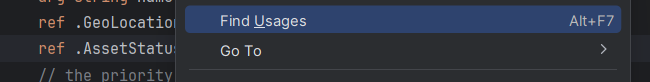
\includegraphics[height=2.5em]{bilder/callReferencen}
        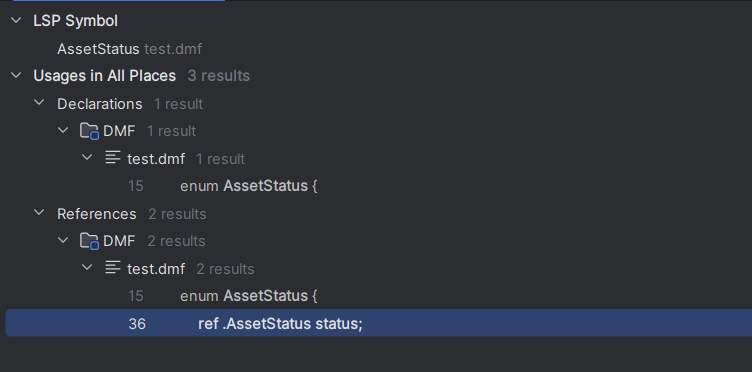
\includegraphics[height=6em]{bilder/referencen}
        \caption{Aufruf der Referenzen}
        \label{fig:callreferencen}
    \end{figure}

    \subsubsection{Faltbereiche}
    Damit Entwickler*innen in großen Dateien die Übersicht behalten können unterstützt der \acrshort{lsp}-Server die Übermittlung von Faltbereichen.
    Die Steuerung der Faltbereiche ist \acrshort{ide} spezifisch.
    \begin{figure}[H]
        \centering
        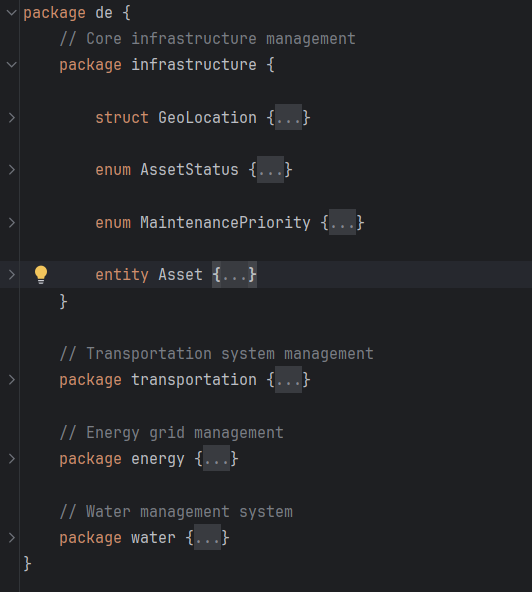
\includegraphics[height=15em]{bilder/faltbereich}
        \caption{Nutzung der Faltbereiche}
        \label{fig:faltbereich}
    \end{figure}

    \subsubsection{Auswahlbereiche}
    Damit die Entwickler*innen auch verschiedene Elemente gut Auswählen können, werden die Auswahlbereiche von \acrshort{lsp}-Server berechnet.
    \begin{figure}[H]
        \centering
        $\vimage{bilder/selection1.png}\vpointer
        \vimage{bilder/selection2.png}\vpointer
        \vimage{bilder/selection3.png}\vpointer
        \vimage{bilder/selection4.png}\vpointer
        \vimage{bilder/selection5.png}$
        \caption{Nutzung der Faltbereiche}
        \label{fig:selection}
    \end{figure}

    \section{Nutzung des \acrshort{dmf}}\label{sec:nutzung-des-dmf}
    Zum Darstellen der Benutzung des \acrshort{dmf} wird das Anlegen eines Projektes mit einem Java und einen Typescript Programm beschrieben.


    \dirtree{%
    .1 spam.
    .2 ham.
    .2 eggs.
    .3 more spam.
    .3 dead parrots.
    }


\end{document}